% options:
% thesis=B bachelor's thesis
% thesis=M master's thesis
% czech thesis in Czech language
% slovak thesis in Slovak language
% english thesis in English language
% hidelinks remove colour boxes around hyperlinks

\documentclass[thesis=M,czech,hidelinks]{FITthesis}[2013/05/06]

\usepackage[utf8]{inputenc} % LaTeX source encoded as UTF-8

\usepackage{pdfpages}

\usepackage{graphicx} %graphics files inclusion
% \usepackage{amsmath} %advanced maths
% \usepackage{amssymb} %additional math symbols

\usepackage{dirtree} %directory tree visualisation

% % list of acronyms
% \usepackage[acronym,nonumberlist,toc,numberedsection=autolabel]{glossaries}
% \iflanguage{czech}{\renewcommand*{\acronymname}{Seznam pou{\v z}it{\' y}ch zkratek}}{}
% \makeglossaries

\newcommand{\tg}{\mathop{\mathrm{tg}}} %cesky tangens
\newcommand{\cotg}{\mathop{\mathrm{cotg}}} %cesky cotangens

\setcounter{tocdepth}{2}
\usepackage{listings}
\usepackage{multirow}
\usepackage{hyperref}
\usepackage{subcaption}
\usepackage{graphicx} 
\usepackage{epstopdf}
\usepackage{minted}
\usepackage{tcolorbox}
\usepackage{etoolbox}
\BeforeBeginEnvironment{minted}{\begin{tcolorbox}}%
\AfterEndEnvironment{minted}{\end{tcolorbox}}%

\usepackage{xcolor}
%\let\oldtexttt\texttt
%\renewcommand{\texttt}[2][blue]{\textcolor{#1}{\ttfamily #2}}

%\usemintedstyle{borland}

% % % % % % % % % % % % % % % % % % % % % % % % % % % % % % 
% ODTUD DAL VSE ZMENTE
% % % % % % % % % % % % % % % % % % % % % % % % % % % % % % 

\department{Katedra řídicí techniky}
\title{Automatizovaný systém stahování webového obsahu potřebného k doplňování cleansetu}
\authorGN{Michal} %(křestní) jméno (jména) autora
\authorFN{Staněk} %příjmení autora
\authorWithDegrees{Michal Staněk} %jméno autora včetně současných akademických titulů
\supervisor{Ing. Jan Kubr, Ph.D.}
\acknowledgements{Chtěl bych poděkovat panu Ing. Janu Kubrovi, Ph.D. za odborné vedení mé práce, za pomoc a věcné rady při zpracování této práce.}
\abstractCS{TODO}
\abstractEN{TODO}
\placeForDeclarationOfAuthenticity{V~Praze}
\declarationOfAuthenticityOption{4} %volba Prohlášení (číslo 1-6)
\keywordsCS{Python, Virtualbox, Fiddler, html, js}
\keywordsEN{Python, Virtualbox, Fiddler, html, js}
% \website{http://site.example/thesis} %volitelná URL práce, objeví se v tiráži - úplně odstraňte, nemáte-li URL práce

\begin{document}

% \newacronym{CVUT}{{\v C}VUT}{{\v C}esk{\' e} vysok{\' e} u{\v c}en{\' i} technick{\' e} v Praze}
% \newacronym{FIT}{FIT}{Fakulta informa{\v c}n{\' i}ch technologi{\' i}}



\definecolor{mygreen}{rgb}{0,0.6,0}
\definecolor{mygray}{rgb}{0.95,0.95,0.95}
\definecolor{mymauve}{rgb}{0.58,0,0.82}

\lstset{ %
  xleftmargin=10pt,xrightmargin=10pt,
  frame=tbrl,
  framerule=1pt,
  language=Java,
  backgroundcolor=\color{mygray},   % choose the background color  
  commentstyle=\color{mygreen},    % comment style
  escapeinside={\%*}{*)},          % if you want to add LaTeX within your code
  keywordstyle=\color{blue},       % keyword style
  stringstyle=\color{mymauve},     % string literal style
} 
%\setlength{\parskip}{10pt}

\chapter{Úvod}
Dnešní doba je plná rizik, která představují hrozbu pro každodenního uživatele internetu. Ať už se jedná o phishing (zisk citlivých údajů pomocí podvodné internetové komunikace) či různé druhy malwaru (nežádoucí programy mající za úkol poškodit uživatele). V boji s těmito riziky je důležité chránit sebe a svoje data pomocí antivirových programů. Jedním z nejrozšířenějších je Avast, který má přes 435 milionů aktivních uživatelů a měsíčně zabrání okolo 2 miliardám útoků\cite{avast_flier}.

\section{Motivace}
Avast, stejně jako většina antivirových programů, uchovává informace o všech známých škodlivých entitách. Tato databáze se denně rozšiřuje o spousty nových záznamů, které obsahují nejen informace o celých souborech, ale i kusy kódu webového obsahu (tzv. string detekce), které jsou považovány za příznak podvodných úmyslů. Může se však stát, že je tento kus kódu moc obecný a dochází tak i k blokování čistého obsahu (tzv. fals-positive detekcím). Aby se těmto situacím předcházelo, je zapotřebí udržovat i databázi s čistými záznamy (tzv. cleanset). Tyto záznamy jsou převážně HTML a js soubory.

Dříve, než se nová string detekce začlení do jádra antiviru, je její obsah porovnán se všemi záznamy na cleansetu a pokud dojde ke shodě (tj. detekční string je součástí nějakého souboru na cleansetu), je tato detekce považována za nevalidní. Tímto dochází k zabránění fals-positive detekcím. 

Ideálním stavem je tedy mít záznam o veškerém čistém obsahu internetu, což je samozřejmě nemožné. Avšak čím více záznamů cleanset obsahuje, tím kvalitnější je běh antivirového programu. V současné době dochází k doplňování cleansetu pouze občasně a to převážně manuálně za pomoci jednoduchých scriptů.

\section{Cíle práce} 
 Hlavním cílem této práce je vytvořit plně automatizovaný systém, který bude databázi s čistými záznamy periodicky doplňovat o nový obsah, čímž by mělo dojít ke zlepšení funčnosti antivirového programu. Dále bude potřeba systém začlenit do již stávající  infrastruktury. Primárním úkolem je tedy vytvořit projekt, který by modernizoval doplňování cleansetu, avšak současně je možné systém zobecnit k využití i v jiných aplikacích. Systému bylo dáno kódové označení \textit{Magpie} (česky Straka), protože systém, stejně jako straky, bude shromažďovat data z různých míst a ukládat je na jedno místo. Celý proces bude řádně otestovaný a bude zhodnocen jeho přínos.


\chapter{Analýza a řešení problému}
Jednotlivé body práce by se daly rozdělit na vícero dílčích podproblémů:

\begin{itemize}
	\item Výběr programovacícho jazyka
	\item Předzpracování zadaných adres webových stránek
	\item Zisk čistých souborů z webových stránek
	\item Zabezpečení stahovacího procesu
	\item Nahrání získaného obsahu do databáze cleansetu
	\item Začlenění do stávající infrastruktury
\end{itemize}

\section{Výběr programovacího jazyka}
Podle prvních odhadů a požadavků bude práce obsahovat více odlišných částí, které by měly být jednoduše ovladatelné a propojitelné. K tomu by šlo využít programovacího jazyka \textit{Python}(\ref{sec:python}), který obsahuje velké množství dostupných knihoven. Tato volba je i v soulady s firemní politikou.





\section{Předzpracování zadaných adres}
Předzpracování zadaných adres  se bude řešit pomocí frontového systému \textit{Kafka}(\ref{sec:kafka}).

Systém by měl reagovat na dva typy vstupů. Prvním vstupem budou adresy s vysokou prevalencí (případem takové adresy může být třeba internetový obchod \url{www.amazon.com}), které budou systému periodicky dodávány z externích modulů. Vstupem ale může být i ručně zadaná adresa či seznam adres v případě, kdy by operátor systému potřeboval na cleanset dodat soubory z webových stránek s menší prevalencí, či, ve více obecném řešení, by potřeboval stáhnout zdrojové soubory cílených webových stránek pro odlišné účely.

V obouch případech se vložené adresy nahrají do frontového systému, odkud se budou postupně odebírat (Obr.\ref{fig:kafka_schema}). Využití \textit{Kafky} má výhodu v již naimplementovaném řešení fronty. Jednou z funkcionalit \textit{Kafky}, které by zde šlo využít, je potvrzování zpracované zprávy po přijetí. Tím dojde k zaručení, že se vždy zpracují všechny zprávy ve frontě. 

\begin{figure}[h]
	\centering
	
\includegraphics[width=9cm]{pictures/kafka.png}
	\caption{Využití frontového systému Kafka}
	\label{fig:kafka_schema}
\end{figure}




\section{Zisk čistých souborů z webových stránek}
Jak bylo zmíněno v předchozí kapitole, lze k zisku čistých souborů přistoupit dvěma způsoby. Jednou z možností je otevírat stránky ve webovém prohlížeči a k zisku souborů použít nástroj \textit{Fiddler}, druhým způsobem je emulace webového prohlížeče v \textit{Pythonu} a stahování zdrojových kódů stránek. 

Další problematikou je ošetření přesměrovávání (tzv. redirecty), které se na spoustě webových stránek používá. Jedna z možností je redirecty neřešit a zabývat se pouze obsahem dané url. To by proces zisku zdrojových souborů usnadnilo. Není to ale příliš robustní řešení. Bylo by tedy rozumné s přesměrováváním webových stránek počítat. 

Také by zde měla být implementována logika selekce pouze HTML a js souborů, ostatní soubory pro funkčnost cleansetu nejsou důležité. To je možné provádět přímo při stahování souborů, nebo vždy pro zdanou adresu stáhnout všechny soubory a selekci provézt následně.

Jednotlivé rozebírané metody zisku čistých souborů z webových stránek jsou tedy následující:
\begin{itemize}
	\item Emulace webového prohlížeče a následné parsování webových stránek 
	\item Spoustění stránek v prohlížeči a zachytávání komunikace Fiddlerem
\end{itemize}

\subsection{Emulace webového prohlížeče} \label{sec:parsing}
Oproti druhé metodě s využitím nástroje \textit{Fiddler} by byla emulace webového prohlížeče bezesporu rychlejší. Pro práci s webovými stránkami v \textit{Pythonu} existuje více knihoven, avšak nejčastěji se používá knihovna \textit{Requests}. Její interface je daleko snazší na použití než u knihovny \textit{Urllib}, jejíž výhodou je pouze fakt, že je již obsažena v základní instalaci \textit{Pythonu} a není nutno ji doinstalovávat. 
\begin{figure}[h]
	\centering
	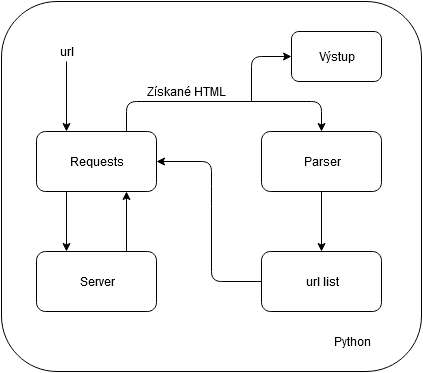
\includegraphics[width=9cm]{pictures/scrapper.png}
	\caption{Diagram zachytávání komunikace pomocí web scrapperu}
	\label{fig:web_scrapper}
\end{figure}
Nevýhoda knihovny \textit{Requests} je v horší práci se stránkami s přesměrováváním pomocí javascriptu nebo obecně s načítáním obsahu pomocí javascriptu. Vytvořit komplexní web scrapper (tj. nástroj, který prochází obsah webových stránek), který by dokázal reagovat i na javascriptem řízený obsah, je netriviální úkol (Obr.\ref{fig:web_scrapper}). 


TODO: mozna trochu popsat netriv ukol requests libky, parsovani html a hledani js scriptu, zminit ze by nebylo nutne pouzivat virtual

\subsection{Zachytávání komunikace Fiddlerem}
Z tohoto důvodu by bylo snazší použít nástroj \textit{Selenium}(\ref{sec:selenium}), čímž už dojde k určitému zpomalení z nutnosti spouštění internetového prohlížeče, avšak odpadne nutnost implementace sledování redirectů a postupného načítání stránek pomocí javascriptu. Stále je ovšem potřeba načtené stránky nějak zpracovat, což by bylo možné pomocí \textit{Fiddleru}(\ref{sec:fiddler}). Tím sice opět vzniká další zpomalení kvůli spouštění dalšího programu, řešení ale přináší téměř kompletní implementaci rozebíraného problému s možnou variací úprav pomocí konfiguračního souboru.
\begin{figure}[h]
	\centering
	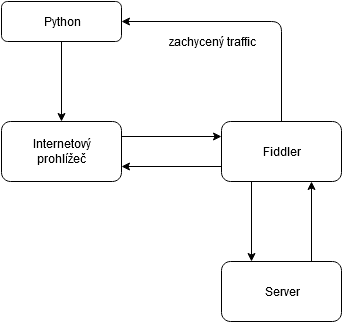
\includegraphics[width=7cm]{pictures/fiddler_diagram.png}
	\caption{Diagram zachytávání komunikace Fiddlerem}
	\label{fig:fiddler}
\end{figure}
Protože je \textit{Fiddler} původně vyvíjen pro testovací účely a sledování internetové komunikace (tzv. traffic), zachytává veškerý traffic, který skrze nástroj proudí (Obr.\ref{fig:fiddler}). Bylo by tedy potřeba implementovat logiku pro třídení a následnou selekci HTML a js souborů.

\subsubsection{Selekce HTML a js souborů}
První přístup, emulace webového prohlížeče, přináší výhodu v tom, že se rovnou při parsování HTML stránek přistupuje pouze k js a HTML souborům, čímž odpadá nutnost následně nějakou selekci provádět. Metoda s použitím \textit{Fiddleru} je v tomto složitější. \textit{Fiddler} je komplexní nástroj a automaticky zachytává veškerou komunikaci - nejen soubory potřebné k vykrelení webové stránky, ale i režijní komunikaci mezi prohlížečem a serverem. Tento přístup je možné změnit pomocí již zmíněného inicializačního scriptu. 

Avšak problémy této metody přináší i webový prohlížeč, kterého se zde využívá. Téměř vždy při spuštění prohlížeče probíhá nevyžádaná komunikace prohlížeče se servery, která je potřeba vytřídit. I zde je možné využít inicializačního scriptu \textit{Fiddleru}, implementovat třídění již při zachytávání komunikace a zachytávat pouze HTML a js soubory ze serverů, které odpovídají zpracovávané url. To ovšem přináší problémy s přesměrováním, které může seznam chtěných serverů libovolně navyšovat, což už by pro inicializační script představovalo nelehký úkol a takové řešení patrně nebude optimální. Druhý způsob je zachytávat HTML a js komunikaci ze všech serverů a selekci řešit až později při zpracování dat v \textit{Pythonu}. Nedostatkem této možnosti je zvýšená náročnost na paměť, kterou představuje zpracovávání více souborů. Předpokládá se ale, že tato nevyžádaná komunikace bude v poměru s chtěnými soubory minimální, tudíž by k výrazné zvýšení náročnosti na paměť dojít nemělo.





\section{Zabezpečení stahovacího procesu}
Z bezpečnostních důvodů je kladen důraz na to, aby byl veškerý proces stahování webového obsahu zabezpečen. Předpokládá se sice, že všechny stažené soubory budou nezavirované, avšak spoléhat se na to není moc bezpečné řešení. Jedním z možných způsobů jak docílit základní bezpečnosti je vytvoření a obsluha virtuálního stroje, na kterém by docházelo ke stahování souborů. 

Celý koncept zabezpečení stahování pomocí virtuálního systému je ovlivněn použitím nástroje \textit{Fiddler}(\ref{sec:fiddler}) pro stahování souborů z webových stránek. Tato metoda by využívala \textit{Fiddler}, který by běžel na pozadí, spolu s prohlížečem, v kterém by byly stránky otevírány a pomocí \textit{Fiddleru} zachytávána komunikace (Obr.\ref{fig:virtualbox}). 
\begin{figure}[h]
	\centering
	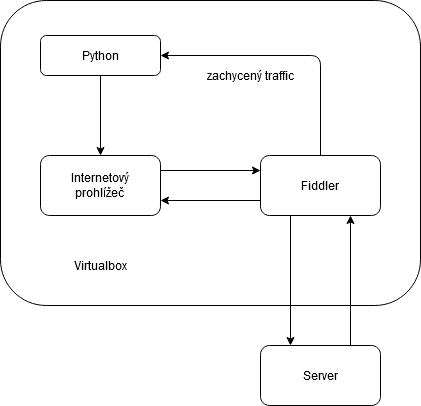
\includegraphics[width=9cm]{pictures/virtualbox.png}
	\caption{Zaobalení stahovacího procesu virtuálním strojem}
	\label{fig:virtualbox}
\end{figure}
Právě otevírání stránek v prohlížeči, během čehož dochází ke spouštění javascriptových souborů, je z pohledu bezpečnosti potenciálně nebezpečné. Toho by se dalo vyvarovat emulací prohlížeče přímo v \textit{Pythonu}, čímž by se stahovaly rovnou zdrojové kódy webových stránek bez nutnosti jejich spouštění. Tato metoda však přináší problémy, které již byly popsané v subsekci \ref{sec:parsing}.

Pokud se jedná o nástroje umožňující virtualizaci systému, lze použít \textit{VMware workstation} od firmy VMware nebo \textit{Virtualbox} vyvíjený firmou Oracle. Firma VMware nabízí pro práci se svými virtuálními stroji infrastrukturu nazývající se \textit{vSphere}. Tato infrastruktura obsahuje vlastní SDK nástroje pro implementaci do programovacího jazyka \textit{Python}\cite{vmware}, avšak celé toto řešení se nenabízí s freeware licencí. Z tohoto důvodu by bylo lepší použít virtualizační nástroj \textit{Virtualbox}(\ref{sec:virtualbox}), který je zdarma. Nevýhoda \textit{Virtualboxu} spočívá v horší podpoře \textit{Pythonu}. Existuje ale knihovna \textit{pyvbox}\cite{pyvbox}, která základní funkčnost podporuje. 

Z hlediska bezpečnosti by bylo rozumné spouštět virtuální stroj (neboli VM) pro každou webovou stránku zvlášť, to by ale celý proces výrazně zpomalovalo. Předpokládá se, že nejdelší dobu zabere právě startování VM.  Jiné řešení by nabízelo restartovat virtuální stroj vždy po určitém čase nebo po daném množství zpracovaných url adres. Tím by se běh systému výrazně zrychlil.





\section{Nahrání získaného obsahu do databáze cleansetu}
Dalším krokem bude přesun získaného obsahu do samotné databáze cleansetu. TODO: scavenger "hdp" dřív samba python client 





\section{Začlenění do stávající infrastruktury}
V současné době se ve společnosti používá pro obdobné projekty systém Jenkins, proto by bylo nejlepší držet se této politiky.






\chapter{Použité technologie}
V této kapitole jsou stručně popsány všechny technologie využité při zpracovávání této práce.
\section{Python 3.7}\label{sec:python}
Python je skriptovací programovací jazyk, jehož syntaxe je lehce odlišná od konvenčních programovacích jazyků (Java, C) v tom, že nepoužívá středníky ani složené závorky. Jedná se o hybridní programovací jazyk, což znamená, že program nemusí být nutně objektově orientovaný, ale části mohou mít více procedurální charakter. Tím dochází k lepší čitelnosti kódu a celkovému zjednodušení. Síla Pythonu je i ve velkém množství balíků s knihovnami, které podporují jeho všestrannost. Kvůli těmto vlastnostem byl vybrán pro tuto diplomovou práci.

\section{Fiddler}\label{sec:fiddler}
Fiddler je nástroj vyvíjen firmou Telerik, sloužící k zachytávání internetové komunikace. Funguje na principu MitM (Man-in-the-middle) útoku, kdy se útočník vtěsná mezi dva účastníky internetového provozu a nechá je komunikovat skrz sebe. Zde je však tento útok chtěný (Obr.\ref{fig:mitm}).
\begin{figure}[h]
	\centering
	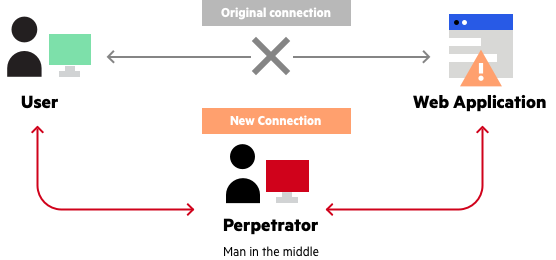
\includegraphics[width=7cm]{pictures/mitm.png}
	\caption{MitM útok \cite{mitm}}
	\label{fig:mitm}
\end{figure}
Jeho automatizace lze docílit inicializačním souborem, který obsahuje různá pravidla a je psaný v javascriptu. Při správném nastavení je fiddler schopný zachytávat i šifrovanou komunikaci, kvůli čemuž byl použit v této práci.

\section{Selenium} \label{sec:selenium}
Selenium je opensource nástroj používaný k automatizovanému přístupu k webovým aplikacím. Těchto vlastností se často využívá při testování, avšak v této práci je použit pouze k obsluze webového prohlížeče. Selenium obsahuje vlastní vývojové prostředí, které lze využít bez velké znalosti programování, existují však i jeho implementace do většiny populárních programovacích jazyků.


\section{Jenkins}
Jenkins je opensource CI/CD systém (continuous integration and delivery) umožňující vykonávání automatických či periodických operací (tzv. jobů). Používá se převážně k spouštění buildů a udržování testů. Joby lze spoustět automaticky po vzniku nové verze vyvíjeného programu, lze je ale i spouštět pravidelně v předem určený čas, čehož bylo v této práci využito.

\section{Kafka}\label{sec:kafka}
Kafka by se dala zařadit mezi frontové systémy. Jedná se o opensource platformu sloužící ke streamování dat v reálném čase. Její zaměření je převážně na procesing velkého množství zpráv bez narůstající latence. Zprávy se však neukládají do fronty, jako je tomu třeba u RabbitMQ (tj. jiný frontový systém), avšak do tzv. topiců. Jeden Topic může obsahovat více částí (tzv. partition), do kterých se zprávy distribuují (Obr.\ref{fig:kafka}). 
\begin{figure}[h]
	\centering
	
\includegraphics[width=7cm]{pictures/kafka.png}
	\caption{Znázornění Kafka systému \cite{kafka}}
	\label{fig:kafka}
\end{figure}
Zprávy do topicu posílá proces, který se nazývá Producer. Obdobně proces, který data čte, je nazýván Consumer. Ten dostává zprávy z topicu v závislosti na indexaci a časové známky. K jednomu topicu může být přihlášeno více nezávislých konzumerů, kteří jsou rozděleni do rozdílných skupin a každá skupina dostává identické zprávy, čím se zabrání vzájemnému čtení stejných zpráv.

Zprávy zůstávají v topicu po určitou dobu, což určuje hodnota retence. Po tuto dobu jsou zprávy přístupny pro každou skupinu konzumerů. Síla kafku je v politice přečtených zpráv. Na rozdíl od zmiňovaného RabbitMQ, který přečtením zprávy zprávu odstraní ze své fronty, funguje v kafce tzv. potvrzovací systém. Konzumer dostane zprávu, a po jejím zpracování vyšle tzv. commit, kterým oznámí úspěšné zpracování. Pokud by v průběhu nastala chyba, tento commit se nepošle a zpráva se vrátí zpátky, kde může být přečtena jiným konzumerem ve skupině.

\section{Virtualbox}\label{sec:virtualbox}
Virtualbox je opensource virtualizační nástroj vyvíjen firmou Oracle. 






\chapter{Implementace}






\chapter{Otestování a zhodnocení přínosu}


 \setlength{\parskip}{10pt}

\begin{conclusion}

\end{conclusion}

\bibliographystyle{csn690}
\bibliography{mybibliographyfile}
\begin{thebibliography}{9}

    \bibitem{avast_flier}
    \textit{Avast corporate factsheet}, Dostupné z: \\       \url{https://cdn2.hubspot.net/hubfs/2706737/media-materials/corporate-factsheet/Avast_corporate_factsheet_A4_en.pdf} \\
       	
    \bibitem{jan}
       	Moravec Jan. \textit{Distribuované řízení kolon vozidel na autodráze}. \textcopyright2014, České vysoké učení technické v Praze, vedoucí práce Ing. Ivo Herman, Dostupné z: \\    \url{https://dspace.cvut.cz/bitstream/handle/10467/24299/F3-BP-2014-Moravec-Jan-prace.pdf} \\
       	
    \bibitem{mitm}
    \url{https://www.imperva.com/learn/application-security/man-in-the-middle-attack-mitm/}


	\bibitem{kafka}
	\url{https://en.wikipedia.org/wiki/Apache_Kafka#/media/File:Overview_of_Apache_Kafka.svg}
	
	\bibitem{vmware}
	\url{[https://code.vmware.com/web/sdk/6.7/vsphere-automation-python]}
	
	\bibitem{pyvbox}
	Dorman Michael. \textit{pyvbox Documentation}. \textcopyright2017 Dostupné z: \\
	\url{https://buildmedia.readthedocs.org/media/pdf/pyvbox/latest/pyvbox.pdf}
	
\end{thebibliography}

\appendix

%\begin{figure}[h]               
%	\begin{minted}{c}
%	code
%	\end{minted}      
%	\caption{Implementace bloku PI regulátor v jazyce C}
%	\label{fig:ctrl.c}
%\end{figure}

%\begin{figure}[h]               
%	\begin{minted}{Java}
%	code
%	\end{minted}      
%	\caption{Deklarace nativní metody a načtení sdílené knihovny}
%	\label{fig:SISO.java}
%\end{figure}

% \begin{figure}[h]
%         \centering
%         \begin{minipage}[b]{0.49\textwidth}
%                 \includegraphics[width=6cm]{pictures/car2.JPG}
%                 \caption*{(a) Pohled po odmontování kapoty}
%                 \label{fig:car2}
% 		\end{minipage}
%         \begin{minipage}[b]{0.49\textwidth}
%                 \includegraphics[width=6cm]{pictures/car3.JPG}
%                 \caption*{(b) Spodní STM modul a DC motor}
%                 \label{fig:car1}
%         \end{minipage}
% 	\caption{Vnitřek vozidel}
% 	\label{fig:cars}
% \end{figure}

%\chapter{Seznam použitých zkratek}
% \printglossaries
%\begin{description}
%	\item[GUI] Graphical user interface
%	\item[XML] Extensible markup language
%\end{description}


% % % % % % % % % % % % % % % % % % % % % % % % % % % % 
% % Tuto kapitolu z výsledné práce ODSTRAŇTE.
% % % % % % % % % % % % % % % % % % % % % % % % % % % % 
% 
% \chapter{Návod k~použití této šablony}
% 
% Tento dokument slouží jako základ pro napsání závěrečné práce na Fakultě informačních technologií ČVUT v~Praze.
% 
% \section{Výběr základu}
% 
% Vyberte si šablonu podle druhu práce (bakalářská, diplomová), jazyka (čeština, angličtina) a kódování (ASCII, \mbox{UTF-8}, \mbox{ISO-8859-2} neboli latin2 a nebo \mbox{Windows-1250}). 
% 
% V~české variantě naleznete šablony v~souborech pojmenovaných ve formátu práce\_kódování.tex. Typ může být:
% \begin{description}
% 	\item[BP] bakalářská práce,
% 	\item[DP] diplomová (magisterská) práce.
% \end{description}
% Kódování, ve kterém chcete psát, může být:
% \begin{description}
% 	\item[UTF-8] kódování Unicode,
% 	\item[ISO-8859-2] latin2,
% 	\item[Windows-1250] znaková sada 1250 Windows.
% \end{description}
% V~případě nejistoty ohledně kódování doporučujeme následující postup:
% \begin{enumerate}
% 	\item Otevřete šablony pro kódování UTF-8 v~editoru prostého textu, který chcete pro psaní práce použít -- pokud můžete texty s~diakritikou normálně přečíst, použijte tuto šablonu.
% 	\item V~opačném případě postupujte dále podle toho, jaký operační systém používáte:
% 	\begin{itemize}
% 		\item v~případě Windows použijte šablonu pro kódování \mbox{Windows-1250},
% 		\item jinak zkuste použít šablonu pro kódování \mbox{ISO-8859-2}.
% 	\end{itemize}
% \end{enumerate}
% 
% 
% V~anglické variantě jsou šablony pojmenované podle typu práce, možnosti jsou:
% \begin{description}
% 	\item[bachelors] bakalářská práce,
% 	\item[masters] diplomová (magisterská) práce.
% \end{description}
% 
% \section{Použití šablony}
% 
% Šablona je určena pro zpracování systémem \LaTeXe{}. Text je možné psát v~textovém editoru jako prostý text, lze však také využít specializovaný editor pro \LaTeX{}, např. Kile.
% 
% Pro získání tisknutelného výstupu z~takto vytvořeného souboru použijte příkaz \verb|pdflatex|, kterému předáte cestu k~souboru jako parametr. Vhodný editor pro \LaTeX{} toto udělá za Vás. \verb|pdfcslatex| ani \verb|cslatex| \emph{nebudou} s~těmito šablonami fungovat.
% 
% Více informací o~použití systému \LaTeX{} najdete např. v~\cite{wikilatex}.
% 
% \subsection{Typografie}
% 
% Při psaní dodržujte typografické konvence zvoleného jazyka. České \uv{uvozovky} zapisujte použitím příkazu \verb|\uv|, kterému v~parametru předáte text, jenž má být v~uvozovkách. Anglické otevírací uvozovky se v~\LaTeX{}u zadávají jako dva zpětné apostrofy, uzavírací uvozovky jako dva apostrofy. Často chybně uváděný symbol "{} (palce) nemá s~uvozovkami nic společného.
% 
% Dále je třeba zabránit zalomení řádky mezi některými slovy, v~češtině např. za jednopísmennými předložkami a spojkami (vyjma \uv{a}). To docílíte vložením pružné nezalomitelné mezery -- znakem \texttt{\textasciitilde}. V~tomto případě to není třeba dělat ručně, lze použít program \verb|vlna|.
% 
% Více o~typografii viz \cite{kobltypo}.
% 
% \subsection{Obrázky}
% 
% Pro umožnění vkládání obrázků je vhodné použít balíček \verb|graphicx|, samotné vložení se provede příkazem \verb|\includegraphics|. Takto je možné vkládat obrázky ve formátu PDF, PNG a JPEG jestliže používáte pdf\LaTeX{} nebo ve formátu EPS jestliže používáte \LaTeX{}. Doporučujeme preferovat vektorové obrázky před rastrovými (vyjma fotografií).
% 
% \subsubsection{Získání vhodného formátu}
% 
% Pro získání vektorových formátů PDF nebo EPS z~jiných lze použít některý z~vektorových grafických editorů. Pro převod rastrového obrázku na vektorový lze použít rasterizaci, kterou mnohé editory zvládají (např. Inkscape). Pro konverze lze použít též nástroje pro dávkové zpracování běžně dodávané s~\LaTeX{}em, např. \verb|epstopdf|.
% 
% \subsubsection{Plovoucí prostředí}
% 
% Příkazem \verb|\includegraphics| lze obrázky vkládat přímo, doporučujeme však použít plovoucí prostředí, konkrétně \verb|figure|. Například obrázek \ref{fig:float} byl vložen tímto způsobem. Vůbec přitom nevadí, když je obrázek umístěn jinde, než bylo původně zamýšleno -- je tomu tak hlavně kvůli dodržení typografických konvencí. Namísto vynucování konkrétní pozice obrázku doporučujeme používat odkazování z~textu (dvojice příkazů \verb|\label| a \verb|\ref|).
% 
% \begin{figure}\centering
% 	
\includegraphics[width=0.5\textwidth, angle=30]{cvut-logo-bw}
% 	\caption[Příklad obrázku]{Ukázkový obrázek v~plovoucím prostředí}\label{fig:float}
% \end{figure}
% 
% \subsubsection{Verze obrázků}
% 
% % Gnuplot BW i barevně
% Může se hodit mít více verzí stejného obrázku, např. pro barevný či černobílý tisk a nebo pro prezentaci. S~pomocí některých nástrojů na generování grafiky je to snadné.
% 
% Máte-li například graf vytvořený v programu Gnuplot, můžete jeho černobílou variantu (viz obr. \ref{fig:gnuplot-bw}) vytvořit parametrem \verb|monochrome dashed| příkazu \verb|set term|. Barevnou variantu (viz obr. \ref{fig:gnuplot-col}) vhodnou na prezentace lze vytvořit parametrem \verb|colour solid|.
% 
% \begin{figure}\centering
% 	\includegraphics{gnuplot-bw}
% 	\caption{Černobílá varianta obrázku generovaného programem Gnuplot}\label{fig:gnuplot-bw}
% \end{figure}
% 
% \begin{figure}\centering
% 	\includegraphics{gnuplot-col}
% 	\caption{Barevná varianta obrázku generovaného programem Gnuplot}\label{fig:gnuplot-col}
% \end{figure}
% 
% 
% \subsection{Tabulky}
% 
% Tabulky lze zadávat různě, např. v~prostředí \verb|tabular|, avšak pro jejich vkládání platí to samé, co pro obrázky -- použijte plovoucí prostředí, v~tomto případě \verb|table|. Například tabulka \ref{tab:matematika} byla vložena tímto způsobem.
% 
% \begin{table}\centering
% 	\caption[Příklad tabulky]{Zadávání matematiky}\label{tab:matematika}
% 	\begin{tabular}{|l|l|c|c|}\hline
% 		Typ		& Prostředí		& \LaTeX{}ovská zkratka	& \TeX{}ovská zkratka	\tabularnewline \hline \hline
% 		Text		& \verb|math|		& \verb|\(...\)|	& \verb|$...$|		\tabularnewline \hline
% 		Displayed	& \verb|displaymath|	& \verb|\[...\]|	& \verb|$$...$$|	\tabularnewline \hline
% 	\end{tabular}
% \end{table}
% 
% % % % % % % % % % % % % % % % % % % % % % % % % % % % 

\chapter{Obsah přiloženého CD}

%upravte podle skutecnosti

\begin{figure}
	\dirtree{%
		.1 slotcar-sw\DTcomment{adresář s Java projektem}.
		.1 SimulinkControllers.
		.2 SISO\DTcomment{jednovstupový regulátor}.
		.2 TwoInputSingleOutput\DTcomment{dvouvstupový regulátor}.
		.2 MISO\DTcomment{vícevstupový regulátor}.
		.2 transferscript.bat\DTcomment{skript pro přenos souborů}.
		.1 text.
		.2 thesis.pdf\DTcomment{text práce ve formátu PDF}.
		.2 thesis.tex\DTcomment{text práce ve formátu \LaTeX}.
		.2 pictures\DTcomment{zdrojové obrázky pro formát \LaTeX}.
		.1 video.
		.2 tutorial.mp4\DTcomment{instruktážní video}.
	}
\end{figure}

\end{document}
